\documentclass{article}
\linespread{1.3}
\usepackage[margin=50pt, headheight=100pt, headsep=0pt]{geometry}
\usepackage{amsmath, amssymb, amsthm, tikz, fancyhdr, float, graphicx, spverbatim, systeme}
\pagestyle{fancy}
\renewcommand{\headrulewidth}{0pt}
\newcommand{\changefont}{\fontsize{15}{15}\selectfont}

\fancypagestyle{firstpageheader}{
  \fancyhead[R]{
    \changefont
    \parbox[t]{4cm}{ % Adjust width as needed
      Michael Huang\\
      EN.625.740.81\\
      Midterm
    }
  }
}

\begin{document}

\thispagestyle{firstpageheader}
{\Large 

\section*{1.}
Recall that if \(f(\mathbf{x})\) and \(g(\mathbf(x))\) are probability distributions, then the Kullback-Leibler divergence of \(g\) from \(f\) is 
\[
  D(f, g) = \int_{-\infty}^{\infty} \dots \int_{-\infty}^{\infty} f(\mathbf{x}) \log [\frac{f(\mathbf{x})}{g(\mathbf{x})}] d \mathbf{x}. 
\]


}
{\Large 

\section*{2.}
The columns in the file \texttt{midterm\_exam\_data.txt} are the \(X\) and \(Y\) values of a function which is a sum of cosines with added Gaussian noise.

\subsection*{(a)}
For various values of \(n\), fit an \(n^{\text{th}}\) order cosine series \((y = \frac{a_0}{2} + \sum_{k=1}^{n} a_k \cos kx)\) to the data. What would you say is the most likely value of \(n\)? \\ \\


\subsection*{(b)}
Estimate the level of the noise. \\ \\


}
{\Large 

\section*{3.}
Consider a Bayesian classifier, with distributions being \(n\)-dimensional multivariate Bernoulli random variables. The conditional probability for a given category is 
\[
  P(\mathbf{x} | \boldsymbol{\theta}) = \prod_{i=1}^{n} \theta_i^{x_i} (1 - \theta_i)^{1 - x_i},
\]
and let \(\mathcal{D} = \{\mathbf{x}_1, \dots, \mathbf{x}_k\}\) be a set of \(k\) samples independently drawn from this probability density. 

\subsection*{(a)} 
If \(\mathbf{s} = (s_1, \dots, s_n)^T\) is the sum of the \(k\) samples, show that 
\[
  P(\mathcal{D} | \boldsymbol{\theta}) = \prod_{i=1}^{n} \theta_i^{s_i} (1 - \theta_i)^{k - s_i},
\] \\
With the setup of the problem with independent samples drawn from a Bernoulli distribution, this is simply the likelihood function. We can therefore just express this as the product of the probability densities:
\[
  P(\mathcal{D} | \boldsymbol{\theta}) = \mathcal{L}(\boldsymbol{\theta} | D) = \prod_{j=1}^{k} P(\mathbf{x}_j | \boldsymbol{\theta})
\]
\[
  = \prod_{j=1}^{k} (\prod_{i=1}^{n} \theta_i^{x_{ij}} (1 - \theta_i)^{1-x_{ij}}) = \prod_{j=1}^{k} \prod_{i=1}^{n} \theta_i^{x_{ij}} (1 - \theta_i)^{1-x_{ij}}
\]
\[
  = \prod_{i=1}^{n} \prod_{j=1}^{k} \theta_i^{x_{ij}} (1 - \theta_i)^{1-x_{ij}}
\]
\[
  = \prod_{i=1}^{n} \theta_i^{\sum_{j=1}^k x_{ij}} (1 - \theta_i)^{\sum_{j=1}^{k} 1-x_{ij}}
\]
Substituting the sum \(s\) in accordingly as given gives us exactly the desired result:
\[
  \boxed{P(\mathcal{D} | \boldsymbol{\theta}) = \prod_{i=1}^{n} \theta_i^{s_i} (1 - \theta_i)^{k - s_i}}
\]

\subsection*{(b)}
Assuming a uniform prior distribution for \(\boldsymbol{\theta}\) show that 
\[
  P(\boldsymbol{\theta} | \mathcal{D}) = \prod_{i=1}^{n} \frac{(k+1)!}{s_i! (k - s_i)!} \theta_i^{s_i} (1 - \theta_i)^{k - s_i},
\] \\
From part (a), we can find this using Bayes' thoerem:
\[
  P(\boldsymbol{\theta} | \mathcal{D}) = \frac{P(\mathcal{D} | \boldsymbol{\theta}) \cdot P(\boldsymbol{\theta})}{P(\mathcal{D})}
\]
\[
  = \frac{P(\mathcal{D} | \boldsymbol{\theta}) \cdot P(\boldsymbol{\theta})}{\int P(\mathcal{D} | \boldsymbol{\theta}) \cdot P(\boldsymbol{\theta})}
\]
Substituting in our result from part (a):
\[
  = \frac{\prod_{i=1}^{n} \theta_i^{s_i} (1 - \theta_i)^{k - s_i} \cdot P(\boldsymbol{\theta})}{\int \prod_{i=1}^{n} \theta_i^{s_i} (1 - \theta_i)^{k - s_i} \cdot P(\boldsymbol{\theta})}
\]
And using the assumption of the uniform distribution for \(\boldsymbol{\theta}\), i.e. \(P(\boldsymbol{\theta}) = 1\) for \(0 \leq \theta_i \leq 1\):
\[
  = \frac{\prod_{i=1}^{n} \theta_i^{s_i} (1 - \theta_i)^{k - s_i} \cdot 1}{\int \prod_{i=1}^{n} \theta_i^{s_i} (1 - \theta_i)^{k - s_i} \cdot 1}
\] 
\[
  = \frac{\prod_{i=1}^{n} \theta_i^{s_i} (1 - \theta_i)^{k - s_i}}{\prod_{i=1}^{n} \int_{0}^{1} \theta_i^{s_i} (1 - \theta_i)^{k - s_i} d\theta_i}
\] 
We use integration by parts in the denominator: \\
- \(u = (1 - \theta_i)^{k - s_i}\) \\
- \(du = (1 - \theta_i)^{k - s_i - 1} \cdot (k - s_i) \cdot -1 d\theta_i = (s_i - k)(1 - \theta_i)^{k - s_i - 1} d\theta_i\)\\
- \(v = \frac{\theta_i^{s_i + 1}}{s_i + 1}\) \\
- \(dv = \theta_i^{si} d\theta_i\)
And substituting accordingly:
\[
  = \frac{\prod_{i=1}^{n} \theta_i^{s_i} (1 - \theta_i)^{k - s_i}}{\prod_{i=1}^{n} (1 - \theta_i)^{k - s_i} \cdot \frac{\theta_i^{s_i + 1}}{s_i + 1} |_{0}^{1} - \int_{0}^{1} \frac{\theta_i^{s_i + 1}}{s_i + 1} \cdot (s_i - k)(1 - \theta_i)^{k - s_i - 1} d \theta_i}
\] 
\[
  = \frac{\prod_{i=1}^{n} \theta_i^{s_i} (1 - \theta_i)^{k - s_i}}{\prod_{i=1}^{n} 0 - 0 - \int_{0}^{1} \frac{\theta_i^{s_i + 1}}{s_i + 1} \cdot (s_i - k)(1 - \theta_i)^{k - s_i - 1} d \theta_i}
\] 
\[
  = \frac{\prod_{i=1}^{n} \theta_i^{s_i} (1 - \theta_i)^{k - s_i}}{\prod_{i=1}^{n} 0 - 0 - \int_{0}^{1} \frac{\theta_i^{s_i + 1}}{s_i + 1} \cdot (s_i - k)(1 - \theta_i)^{k - s_i - 1} d \theta_i}
\]
\[
  = \frac{\prod_{i=1}^{n} \theta_i^{s_i} (1 - \theta_i)^{k - s_i}}{\prod_{i=1}^{n} - \frac{s_i - k}{s_i + 1} \int_{0}^{1} \theta_i^{s_i + 1} (1 - \theta_i)^{k - s_i - 1} d \theta_i}
\]
We can see that from repeatedly applying integration by parts, we eventually reduce the exponent of the \(1 - \theta_i\) term to 0, while the exponent of the \(\theta_i\) term increases until \(k\), giving us:
\[
  = \frac{\prod_{i=1}^{n} \theta_i^{s_i} (1 - \theta_i)^{k - s_i}}{\prod_{i=1}^{n} \frac{(k - s_i) (k - s_i - 1) \dots 1}{(s_i + 1) (s_i + 2) \dots k} \int_{0}^{1} \theta_i^k (1 - \theta_i)^{0} d \theta_i}
\]
\[
  = \frac{\prod_{i=1}^{n} \theta_i^{s_i} (1 - \theta_i)^{k - s_i}}{\prod_{i=1}^{n} \frac{(k - s_i) (k - s_i - 1) \dots 1}{(s_i + 1) (s_i + 2) \dots k} \int_{0}^{1} \theta_i^k (1 - \theta_i)^{0} d \theta_i}
\]
\[
  = \frac{\prod_{i=1}^{n} \theta_i^{s_i} (1 - \theta_i)^{k - s_i}}{\prod_{i=1}^{n} \frac{(k - s_i) (k - s_i - 1) \dots 1}{(s_i + 1) (s_i + 2) \dots k} \int_{0}^{1} \theta_i^k d\theta_i}
\]
\[
  = \frac{\prod_{i=1}^{n} \theta_i^{s_i} (1 - \theta_i)^{k - s_i}}{\prod_{i=1}^{n} \frac{(k - s_i) (k - s_i - 1) \dots 1}{(s_i + 1) (s_i + 2) \dots k} [\frac{\theta_i^{k+1}}{k+1}]_{0}^{1}}
\]
\[
  = \frac{\prod_{i=1}^{n} \theta_i^{s_i} (1 - \theta_i)^{k - s_i}}{\prod_{i=1}^{n} \frac{(k - s_i) (k - s_i - 1) \dots 1}{(s_i + 1) (s_i + 2) \dots k} (\frac{1}{k+1} - 0)}
\]
\[
  = \frac{\prod_{i=1}^{n} \theta_i^{s_i} (1 - \theta_i)^{k - s_i}}{\prod_{i=1}^{n} \frac{(k - s_i)!}{(s_i + 1) (s_i + 2) \dots k+1}}
\]
\[
  = \frac{\prod_{i=1}^{n} \theta_i^{s_i} (1 - \theta_i)^{k - s_i}}{\prod_{i=1}^{n} \frac{(k - s_i)!}{(s_i + 1) (s_i + 2) \dots k+1} \cdot \frac{s_i!}{s_i!}} 
\]
\[
  = \frac{\prod_{i=1}^{n} \theta_i^{s_i} (1 - \theta_i)^{k - s_i}}{\prod_{i=1}^{n} \frac{(k - s_i)!s_i!}{(k+1)!} } 
\]
\[
  = \prod_{i=1}^{n} \frac{\theta_i^{s_i} (1 - \theta_i)^{k - s_i}}{\frac{(k - s_i)!s_i!}{(k+1)!} } 
\]
\[
  \boxed{ P(\boldsymbol{\theta} | \mathcal{D}) = \prod_{i=1}^{n} \frac{(k+1)!}{s_i!(k - s_i)!} \theta_i^{s_i} (1 - \theta_i)^{k - s_i} }
\]
exactly as we sought to find. 

\subsection*{(c)}
Plot this density for the case \(n = 1, k = 1\) and for the two resulting possibilities for \(s_i\). \\ \\
With \(n = 1\), we have one sample, so our only cases are either \(s = 0\) or \(s = 1\): \\
- If \(s=0\), we have 
\[
  P(\boldsymbol{\theta} | \mathcal{D}) = \frac{(1 + 1)!}{0! (1 - 0)!} \cdot \theta^0 \cdot (1 - \theta)^{1 - 0} = \frac{2!}{0!1!} \cdot 1 \cdot (1 - \theta)^1 = 2 - 2\theta
\]
- If \(s=1\), we have 
\[
  P(\boldsymbol{\theta} | \mathcal{D}) = \frac{(1+1)!}{1!(1 - 1)!} \cdot  \theta^1 \cdot (1 - \theta)^{1 - 1} = \frac{2!}{1!0!} \cdot \theta \cdot (1 - \theta)^0 = 2\theta
\]
We plot this below: 
\begin{figure}[h!]
  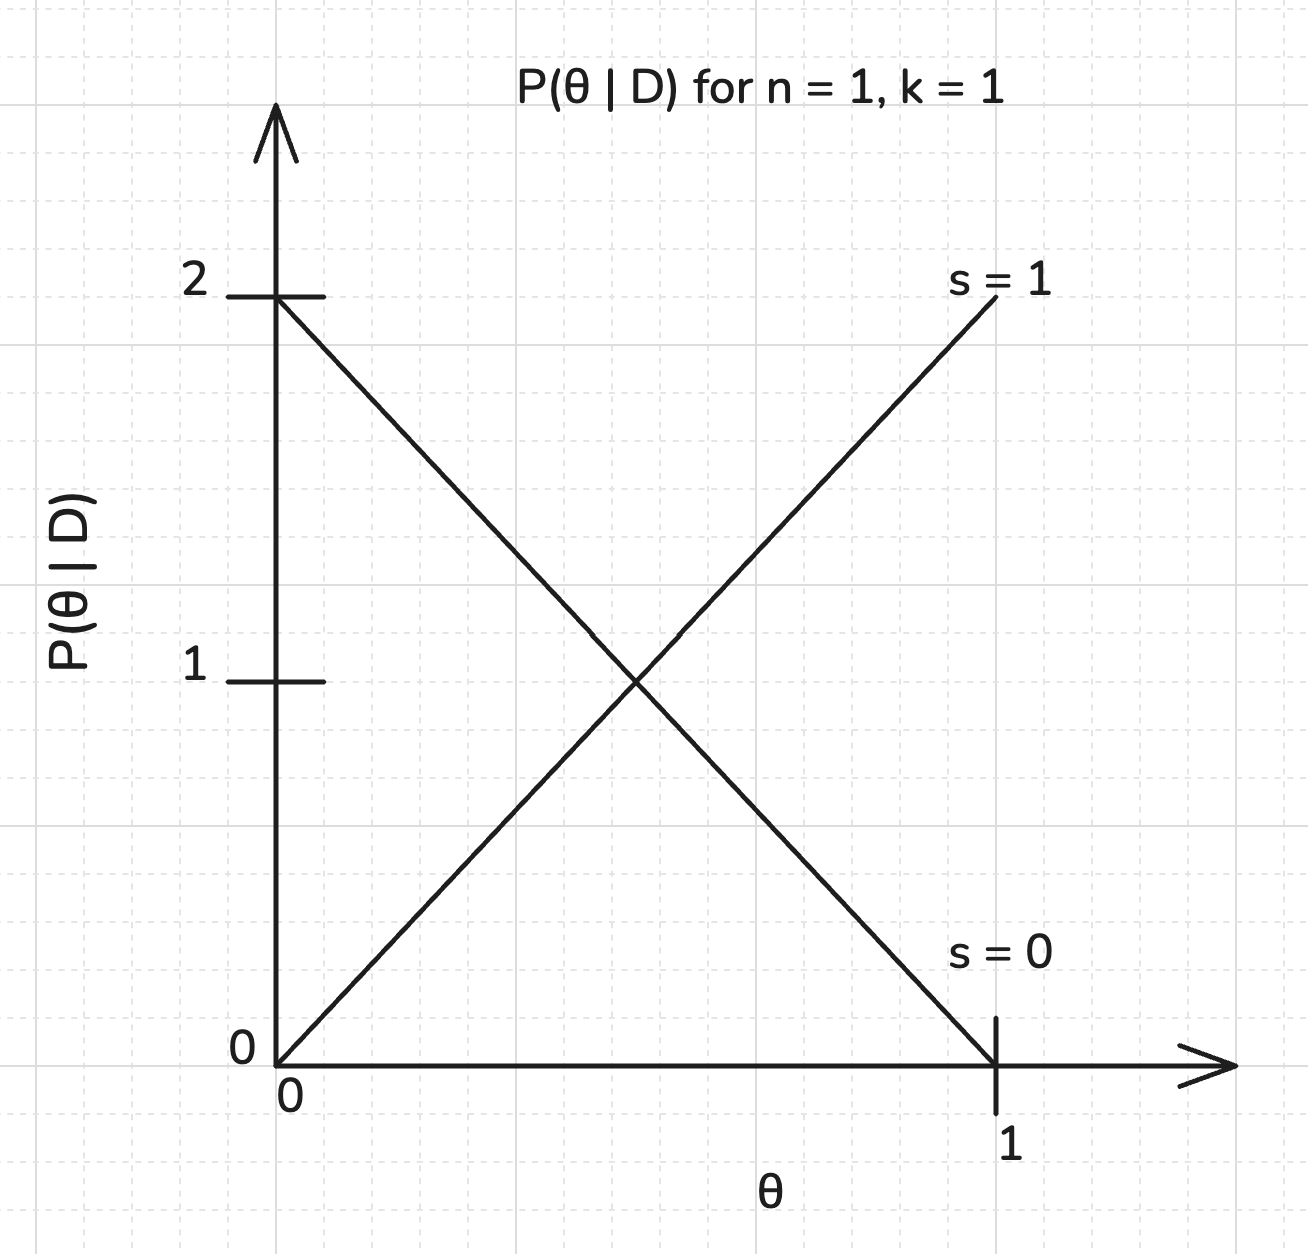
\includegraphics[width=300pt]{problem_3_c.png}
\end{figure}

\subsection*{(d)}
Integrate the product \(P(\mathbf{x} | \boldsymbol{\theta}) P(\boldsymbol{\theta} | \mathcal{D})\) over \(\boldsymbol{\theta}\) to obtain 
\[
  P(\mathbf{x} | \mathcal{D}) = \prod_{i=1}^{n} (\frac{s_i + 1}{k + 2})^{x_i} (1 - \frac{s_i + 1}{k + 1})^{1 - x_i}
\] \\
As directed, we start with
\[
  P(\mathbf{x} | \mathcal{D}) = \int_{\boldsymbol{\theta}} P(\mathbf{x} | \boldsymbol{\theta}) P(\boldsymbol{\theta} | \mathcal{D}) d \boldsymbol{\theta}
\]
Substituting the given conditional probability and our finding from part (b):
\[
  = \int_{\boldsymbol{\theta}} (\prod_{i=1}^{n} \theta_i^{x_i} (1 - \theta_i)^{1 - x_i}) \cdot 
  (\prod_{i=1}^{n} \frac{(k+1)!}{s_i!(k - s_i)!} \theta_i^{s_i} (1 - \theta_i)^{k - s_i}) d \boldsymbol{\theta}
\]
\[
  = \prod_{i=1}^{n} \int_{\boldsymbol{\theta}} \theta_i^{x_i} (1 - \theta_i)^{1 - x_i} \frac{(k+1)!}{s_i!(k - s_i)!} \theta_i^{s_i} (1 - \theta_i)^{k - s_i} d \boldsymbol{\theta}
\]
\[
  = \prod_{i=1}^{n} \frac{(k+1)!}{s_i!(k - s_i)!} \int_{\boldsymbol{\theta}} \theta_i^{x_i} (1 - \theta_i)^{1 - x_i} \theta_i^{s_i} (1 - \theta_i)^{k - s_i} d \boldsymbol{\theta}
\]
\[
  = \prod_{i=1}^{n} \frac{(k+1)!}{s_i!(k - s_i)!} \int_{\boldsymbol{\theta}} \theta_i^{x_i + s_i} (1 - \theta_i)^{k - s_ i - x_i + 1} d \boldsymbol{\theta} 
\]
This leads us into a very similar situation as we saw in part (b) with the repeated integration by parts. In part (b), we have exponents of \(s_i\) and \(k - s_i\); here, we have exponents of \(s_i + x_i\) and \(k - s_i - x_i + 1\), so the \(1 - \theta_i\) term now has 1 additional power relative to the \(\theta_i\) term as it did in part (b). We just integrate by parts \(k - s_i - x_i + 1\) times, giving us 
\[
  = \prod_{i=1}^{n} \frac{(k+1)!}{s_i!(k - s_i)!} \cdot \frac{(k - s_i - x_i + 1)!}{(s_i + x_i + 1) (x_i + s_i + 2) \dots (k + 1)} \int_{0}^{1} \theta_i^{k+1} (1 - \theta_i)^{0} d \boldsymbol{\theta} 
\]
\[
  = \prod_{i=1}^{n} \frac{(k+1)!}{s_i!(k - s_i)!} \cdot \frac{(k - s_i - x_i + 1)!}{(s_i + x_i + 1) (x_i + s_i + 2) \dots (k + 1)} [\frac{\theta_i^{k+2}}{k+2}]_0^{1} 
\]
\[
  = \prod_{i=1}^{n} \frac{(k+1)!}{s_i!(k - s_i)!} \cdot \frac{(k - s_i - x_i + 1)!}{(s_i + x_i + 1) (x_i + s_i + 2) \dots (k + 1)} \cdot (\frac{1}{k+2} - 0)
\]
\[
  = \prod_{i=1}^{n} \frac{(k+1)!}{s_i!(k - s_i)!} \cdot \frac{(k - s_i - x_i + 1)!}{(s_i + x_i + 1) (x_i + s_i + 2) \dots (k + 2)}
\]
\[
  = \prod_{i=1}^{n} \frac{(k+1)!}{s_i!(k - s_i)!} \cdot \frac{(k - s_i - x_i + 1)!}{(s_i + x_i + 1) (x_i + s_i + 2) \dots (k + 2)} \cdot \frac{(s_i + x_i)!}{(s_i + x_i)!}
\]
\[
  = \prod_{i=1}^{n} \frac{(k+1)!}{s_i!(k - s_i)!} \cdot \frac{(k - s_i - x_i + 1)!(s_i + x_i)!}{(k+2)!}
\]
\[
  = \prod_{i=1}^{n} \frac{(k - s_i - x_i + 1)!(s_i + x_i)!}{s_i!(k - s_i)!(k+2)}
\]
\[
  = \prod_{i=1}^{n} \frac{(k - s_i - x_i + 1)!(s_i + x_i)!}{s_i!(k - s_i)!(k+2)}
\]
From this point, we can take a hint from the structure of the answer to see that we should be looking at the two different cases for \(x_i\), that is, because it is Bernoulli, it must either be 1 or 0. Looking at these cases: \\
- If \(x_i = 0\), we get
\[
  \frac{(k - s_i - 0 + 1)!(s_i + 0)!}{s_i!(k - s_i)!(k+2)} = \frac{(k - s_i + 1)!s_i!}{s_i!(k - s_i)!(k+2)} = \frac{k - s_i + 1}{k+2}
\]
- If \(x_i = 1\), we get 
\[
  \frac{(k - s_i - 1 + 1)!(s_i + 1)!}{s_i!(k - s_i)!(k+2)} = \frac{s_i + 1}{k+2}
\]
And we then can express this using the exponents to account for the 0 / 1 on/off nature of the results. We therefore get 
\[
  = \prod_{i=1}^{n} (\frac{k - s_i + 1}{k+2})^{1 - x_i} (\frac{s_i + 1}{k+2})^{x_i}
\]
\[
  = \prod_{i=1}^{n} (\frac{s_i + 1}{k+2})^{x_i} (\frac{k - s_i + 1}{k+2})^{1 - x_i} 
\]
\[
  = \prod_{i=1}^{n} (\frac{s_i + 1}{k+2})^{x_i} (\frac{k + 2 - s_i - 1}{k+2})^{1 - x_i} 
\]
\[
  \boxed{P(\mathbf{x} | \mathcal{D}) = \prod_{i=1}^{n} (\frac{s_i + 1}{k+2})^{x_i} (1 - \frac{s_i + 1}{k+2})^{1 - x_i} }
\]
exactly as we sought to find.

\subsection*{(e)}
Compare the expressions for \(P(\mathbf{x} | \mathcal{D})\) and \(P(\mathbf{x} | \boldsymbol{\theta}).\) What is \(\hat{\boldsymbol{\theta}}\), the effective Bayesian estimate for \(\boldsymbol{\theta}\)? \\ \\
To recap, we have 
\[
  P(\mathbf{x} | \mathcal{D}) = \prod_{i=1}^{n} (\frac{s_i + 1}{k+2})^{x_i} (1 - \frac{s_i + 1}{k+2})^{1 - x_i} 
\]
and 
\[
  P(\mathbf{x} | \boldsymbol{\theta}) = \prod_{i=1}^{n} \theta_i^{x_i} (1 - \theta_i)^{1 - x_i}
\]
We see that that \(\theta_i\) directly maps to \(\frac{s_i + 1}{k + 2}\) for both the \(\theta_i\) and \(1 - \theta_i\) terms, which indicates to us that \(\hat{\boldsymbol{\theta}}\) is \(\boldsymbol{\theta} = (\theta_1, \theta_2, \dots, \theta_n)^T\) where \(\hat{\theta_i} = \frac{s_i + 1}{k + 2}\).

}


\end{document}